\let\negmedspace\undefined
\let\negthickspace\undefined
\documentclass[journal,12pt,twocolumn]{IEEEtran}
\usepackage{gensymb}
\usepackage{polynom}
\usepackage{amssymb}
\usepackage[cmex10]{amsmath}
\usepackage{amsthm}
\usepackage{stfloats}
\usepackage{bm}
\usepackage{longtable}
\usepackage{enumitem}
\usepackage{mathtools}
\usepackage{tikz}
\usepackage[breaklinks=true]{hyperref}
\usepackage{listings}
\usepackage{color}                                            
\usepackage{array}                                            
\usepackage{longtable}                                        
\usepackage{calc}                                             
\usepackage{multirow}                                         
\usepackage{hhline}                                           
\usepackage{ifthen}                                           
\usepackage{lscape}     
\usepackage{tfrupee}
\DeclareMathOperator*{\Res}{Res}
\DeclareMathOperator*{\equals}{=}
\hyphenation{op-tical net-works semi-conduc-tor}
\def\inputGnumericTable{}                                 
\lstset{
frame=single, 
breaklines=true,
columns=fullflexible
}
\begin{document}
\newtheorem{theorem}{Theorem}[section]
\newtheorem{problem}{Problem}
\newtheorem{proposition}{Proposition}[section]
\newtheorem{lemma}{Lemma}[section]
\newtheorem{corollary}[theorem]{Corollary}
\newtheorem{example}{Example}[section]
\newtheorem{definition}[problem]{Definition}
\newcommand{\BEQA}{\begin{eqnarray}}
\newcommand{\EEQA}{\end{eqnarray}}
\newcommand{\define}{\stackrel{\triangle}{=}}
\newcommand*\circled[1]{\tikz[baseline=(char.base)]{
\node[shape=circle,draw,inner sep=2pt] (char) {#1};}}
\bibliographystyle{IEEEtran}
\providecommand{\mbf}{\mathbf}
\providecommand{\pr}[1]{\ensuremath{\Pr\left(#1\right)}}
\providecommand{\qfunc}[1]{\ensuremath{Q\left(#1\right)}}
\providecommand{\sbrak}[1]{\ensuremath{{}\left[#1\right]}}
\providecommand{\lsbrak}[1]{\ensuremath{{}\left[#1\right.}}
\providecommand{\rsbrak}[1]{\ensuremath{{}\left.#1\right]}}
\providecommand{\brak}[1]{\ensuremath{\left(#1\right)}}
\providecommand{\lbrak}[1]{\ensuremath{\left(#1\right.}}
\providecommand{\rbrak}[1]{\ensuremath{\left.#1\right)}}
\providecommand{\cbrak}[1]{\ensuremath{\left\{#1\right\}}}
\providecommand{\lcbrak}[1]{\ensuremath{\left\{#1\right.}}
\providecommand{\rcbrak}[1]{\ensuremath{\left.#1\right\}}}
\theoremstyle{remark}
\newtheorem{rem}{Remark}
\newcommand{\sgn}{\mathop{\mathrm{sgn}}}
\providecommand{\fourier}{\overset{\mathcal{F}}{ \rightleftharpoons}}
\providecommand{\system}{\overset{\mathcal{H}}{ \longleftrightarrow}}
\newcommand{\solution}{\noindent \textbf{Solution: }}
\newcommand{\cosec}{\,\text{cosec}\,}
\providecommand{\dec}[2]{\ensuremath{\overset{#1}{\underset{#2}{\gtrless}}}}
\newcommand{\myvec}[1]{\ensuremath{\begin{pmatrix}#1\end{pmatrix}}}
\newcommand{\mydet}[1]{\ensuremath{\begin{vmatrix}#1\end{vmatrix}}}
\makeatletter
\@addtoreset{figure}{problem}
\makeatother
\let\StandardTheFigure\thefigure
\let\vec\mathbf
\def\putbox#1#2#3{\makebox[0in][l]{\makebox[#1][l]{}\raisebox{\baselineskip}[0in][0in]{\raisebox{#2}[0in][0in]{#3}}}}
\def\rightbox#1{\makebox[0in][r]{#1}}
\def\centbox#1{\makebox[0in]{#1}}
\def\topbox#1{\raisebox{-\baselineskip}[0in][0in]{#1}}
\def\midbox#1{\raisebox{-0.5\baselineskip}[0in][0in]{#1}}
\title{Assignment-2}
\author{ Aniket Satpute (CS21BTECH11056)}
\graphicspath{{figure/}}
\maketitle
\begin{abstract}
ICSE Class 12 Maths 2017 Q.20(b)
\end{abstract}

% the text begins here

Question 20\\

(b)	From the given data :\\

\begin{table}[h!]
\center
%\resizebox{\columnwidth}{!}
{
\begin{tabular}{|c|c|c|}
\hline
Variable & x & y\\
\hline
Mean & 6 & 8\\
\hline
 Standard Deviation & 4 & 6\\
 \hline
\end{tabular}
}
\end{table}
and correlation coefficient : $\frac{2}{3}$  Find :\\
(i)	 Regression coefficient $ b_{yx} $ and $b_{xy}$\\
(ii) Regression line x on y\\
(ii) Most likely value of x when y = 14\\
\textbf{ Solution : }\\
$\bar{x}$ = 6 , $\bar{y}$ = 8 , $\sigma_{x}$ = 4 , $\sigma_{y}$ = 6 and r = $\frac{2}{3}$\\
\begin{align}
b_{yx} &= r.\frac{\sigma_{y}}{\sigma_{x}}
        = \frac{2}{3}.\frac{6}{4}
        = 1\\
b_{xy} &= r.\frac{\sigma_{x}}{\sigma_{y}}
        = \frac{2}{3}.\frac{4}{6}
        = \frac{4}{9}
\end{align}

Regression equation x on y\\
\begin{align*}
x - \bar{x} &= bxy( y -\bar{y} )\\
x - 6       &= \frac{4}{9} ( y - 8)\\
9x - 54     &= 4y - 32\\
9x - 4y     &= 22
\end{align*}
When y = 14 ,
\begin{align*}
(9x - 4) 14 &= 22\\
         9x &= 78\\
          x &= 8.67
\end{align*}
\begin{figure}[h]
\centering
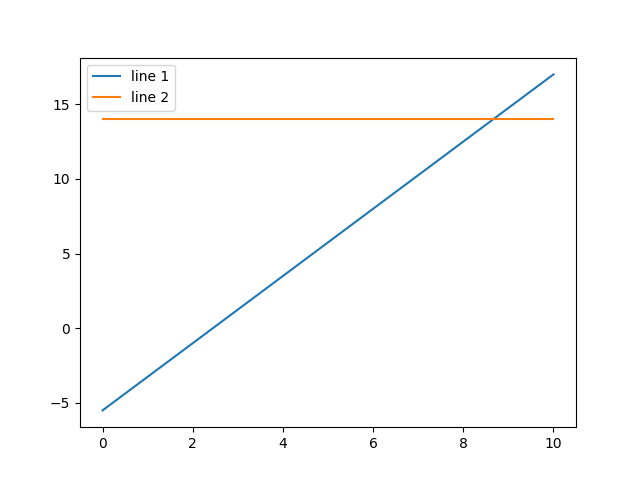
\includegraphics[width=\columnwidth]{fig1.png}
\caption{Finding the intersection point}
\label{Fig1}
\end{figure}
\end{document}